\resizebox{\textwidth}{!}{
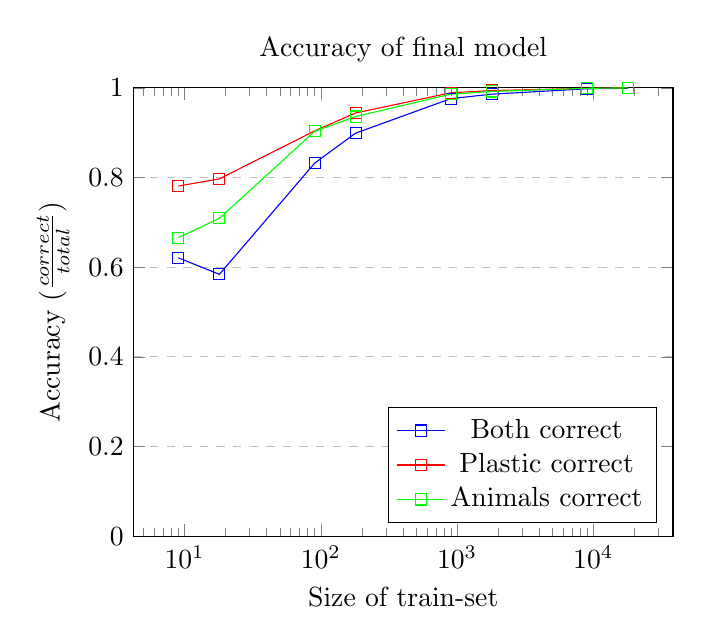
\begin{tikzpicture}
\begin{semilogxaxis}[
    title={Accuracy of final model},
    xlabel={Size of train-set},
    ylabel={Accuracy ($\frac{correct}{total}$)},
    %xmin=0, xmax=18000,
    ymin=0, ymax=1,
    legend pos=south east,
    ymajorgrids=true,
    grid style=dashed,
]
\addplot[
    color=blue,
    mark=square,
    ]
    coordinates {
    (9,0.621)(18,0.584)(90,0.832)(180,0.899)(900,0.976)(1800,0.986)(9000,0.998)(18000,0.999)
    };
    \addlegendentry{Both correct}
\addplot[
    color=red,
    mark=square,
    ]
    coordinates {
    (9,0.781)(18,0.797)(90,0.904)(180,0.944)(900,0.989)(1800,0.994)(9000,0.999)(18000,1.000)
    };
    \addlegendentry{Plastic correct}
\addplot[
    color=green,
    mark=square,
    ]
    coordinates {
    (9,0.666)(18,0.709)(90,0.903)(180,0.936)(900,0.986)(1800,0.992)(9000,0.999)(18000,1.000)
    };
    \addlegendentry{Animals correct}
\end{semilogxaxis}
\end{tikzpicture}
\hspace{.5cm}
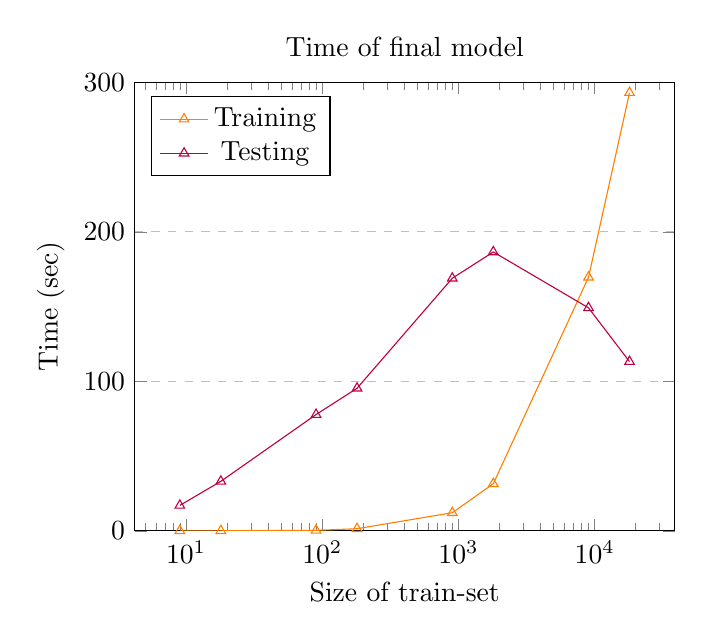
\begin{tikzpicture}
\begin{semilogxaxis}[
    title={Time of final model},
    xlabel={Size of train-set},
    ylabel={Time (sec)},
    %xmin=0, xmax=18000,
    ymin=0, ymax=300,
    legend pos=north west,
    ymajorgrids=true,
    grid style=dashed,
    ]
\addplot[
    color=orange,
    mark=triangle,
    ]
    coordinates {
    (9,0.0)(18,0.0)(90,0.3)(180,1.4)(900,12.1)(1800,31.5)(9000,169.7)(18000,293.2)
    };
    \addlegendentry{Training}
\addplot[
    color=purple,
    mark=triangle,
    ]
    coordinates {
    (9,17.0)(18,33.1)(90,77.8)(180,95.4)(900,169.0)(1800,186.6)(9000,149.2)(18000,113.2)
    };
    \addlegendentry{Testing} 
\end{semilogxaxis}
\end{tikzpicture}
}